\documentclass[aspectratio=169]{beamer}
\usetheme{Madrid}
\usecolortheme{default}

% Packages
\usepackage{graphicx}
\usepackage{amsmath}
\usepackage{amssymb}
\usepackage{booktabs}
\usepackage{algorithm}
\usepackage{algpseudocode}
\usepackage{tikz}
\usetikzlibrary{shapes,arrows,positioning}

% Theme customization
\setbeamertemplate{navigation symbols}{}
\setbeamertemplate{footline}[frame number]

% Title information
\title{Quantum Optimization for Access Point Selection in WiFi Indoor Localization}
\author{Your Name}
\institute{Your Institution}
\date{\today}

\begin{document}

% Slide 1: Title
\begin{frame}
\titlepage
\end{frame}

% Slide 2: Problem Statement
\begin{frame}{Problem Statement}
\begin{columns}
\column{0.6\textwidth}
\textbf{Indoor Localization Challenges:}
\begin{itemize}
    \item WiFi fingerprinting uses \textbf{520 Access Points}
    \item High computational complexity
    \item Signal redundancy and noise
    \item Need for efficient AP selection
\end{itemize}

\vspace{1em}
\textbf{Research Question:}
\begin{quote}
\textit{How can we select an optimal subset of k APs that maximizes localization accuracy while minimizing redundancy?}
\end{quote}

\column{0.4\textwidth}
\begin{center}
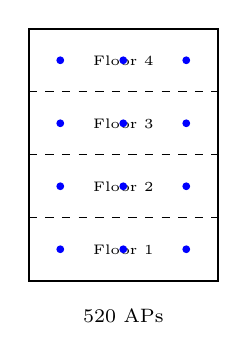
\begin{tikzpicture}[scale=0.8]
    % Building representation
    \draw[thick] (0,0) rectangle (3,4);
    \draw[dashed] (0,1) -- (3,1);
    \draw[dashed] (0,2) -- (3,2);
    \draw[dashed] (0,3) -- (3,3);
    \node at (1.5,3.5) {\tiny Floor 4};
    \node at (1.5,2.5) {\tiny Floor 3};
    \node at (1.5,1.5) {\tiny Floor 2};
    \node at (1.5,0.5) {\tiny Floor 1};

    % APs
    \foreach \y in {0.5,1.5,2.5,3.5} {
        \foreach \x in {0.5,1.5,2.5} {
            \node[circle,fill=blue,inner sep=1pt] at (\x,\y) {};
        }
    }
    \node[below] at (1.5,-0.3) {\scriptsize 520 APs};
\end{tikzpicture}
\end{center}
\end{columns}
\end{frame}

% Slide 3: Objectives
\begin{frame}{Research Objectives}
\begin{block}{Primary Goal}
Optimize Access Point selection using \textbf{Quantum-Inspired Optimization} (QUBO formulation with Simulated Quantum Annealing)
\end{block}

\vspace{1em}
\textbf{Specific Objectives:}
\begin{enumerate}
    \item Reduce AP count from \textbf{520 $\rightarrow$ 20} (96\% reduction)
    \item Maximize localization accuracy (minimize 3D positioning error)
    \item Minimize redundancy between selected APs
    \item Compare multiple feature importance methods
    \item Evaluate quantum-inspired vs. classical solvers
\end{enumerate}

\vspace{0.5em}
\begin{center}
\fbox{\textbf{Key Innovation:} QUBO formulation balancing importance \& redundancy}
\end{center}
\end{frame}

% Slide 4: Dataset
\begin{frame}{Dataset: UJIIndoorLoc}
\begin{columns}
\column{0.5\textwidth}
\textbf{Dataset Statistics:}
\begin{itemize}
    \item \textbf{19,937} training samples
    \item \textbf{1,111} validation samples
    \item \textbf{520} WiFi Access Points
    \item \textbf{3 buildings}, multiple floors
    \item Focus: \textbf{Building 1} (4 floors)
\end{itemize}

\vspace{1em}
\textbf{Features:}
\begin{itemize}
    \item RSSI (Received Signal Strength)
    \item Range: -104 dBm to 0 dBm
    \item 100 = AP not detected
\end{itemize}

\column{0.5\textwidth}
\textbf{Target Variables:}
\begin{itemize}
    \item Longitude (normalized)
    \item Latitude (normalized)
    \item Floor (0-3)
\end{itemize}

\vspace{1em}
\textbf{3D Coordinate System:}
\begin{equation*}
\text{Position} = (\text{LON}_{\text{norm}}, \text{LAT}_{\text{norm}}, \text{FLOOR})
\end{equation*}
\begin{itemize}
    \item Floor height = 3 meters
    \item 3D distance in real-world meters
\end{itemize}
\end{columns}
\end{frame}

% Slide 5: Methodology Overview
\begin{frame}{Methodology Pipeline}
\begin{center}
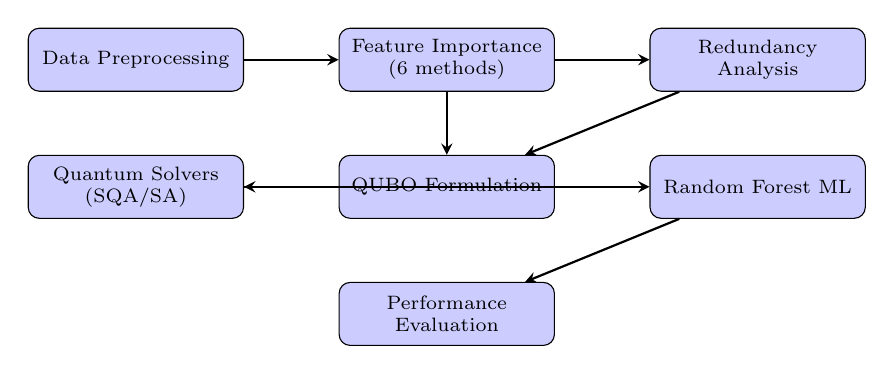
\begin{tikzpicture}[
    node distance=1.2cm,
    block/.style={rectangle, draw, fill=blue!20, text width=2.5cm, text centered, rounded corners, minimum height=0.8cm, font=\scriptsize},
    arrow/.style={thick,->,>=stealth}
]
    \node[block] (data) {Data Preprocessing};
    \node[block, right=of data] (importance) {Feature Importance (6 methods)};
    \node[block, right=of importance] (redundancy) {Redundancy Analysis};

    \node[block, below=0.8cm of importance] (qubo) {QUBO Formulation};
    \node[block, left=of qubo] (solver) {Quantum Solvers (SQA/SA)};
    \node[block, right=of qubo] (ml) {Random Forest ML};

    \node[block, below=0.8cm of qubo] (eval) {Performance Evaluation};

    \draw[arrow] (data) -- (importance);
    \draw[arrow] (importance) -- (redundancy);
    \draw[arrow] (redundancy) -- (qubo);
    \draw[arrow] (importance) -- (qubo);
    \draw[arrow] (qubo) -- (solver);
    \draw[arrow] (solver) -- (ml);
    \draw[arrow] (ml) -- (eval);
\end{tikzpicture}
\end{center}

\vspace{0.5em}
\textbf{Key Steps:}
\begin{enumerate}
    \item Normalize RSSI values to [0,1]
    \item Calculate AP importance using 6 different methods
    \item Compute pairwise redundancy (Pearson correlation)
    \item Formulate QUBO optimization problem
    \item Solve with quantum-inspired annealing
    \item Train Random Forest on selected APs
    \item Evaluate 3D localization accuracy
\end{enumerate}
\end{frame}

% Slide 6: Feature Importance Methods
\begin{frame}{Feature Importance Methods}
\textbf{Six methods to rank 520 Access Points:}

\begin{table}[h]
\centering
\scriptsize
\begin{tabular}{@{}llp{6cm}@{}}
\toprule
\textbf{Method} & \textbf{Formula} & \textbf{Description} \\
\midrule
Entropy & $H(X) = -\sum p(x)\log p(x)$ & Shannon entropy of RSSI distribution \\
Average & $\bar{x} = \frac{1}{n}\sum x_i$ & Mean RSSI value across samples \\
Median & $x_{0.5}$ & Median RSSI (robust to outliers) \\
Max & $\max(x)$ & Maximum RSSI (strongest signal) \\
Variance & $\sigma^2 = \frac{1}{n}\sum (x_i - \bar{x})^2$ & Signal diversity measure \\
Mutual Info & $I(X;Y)$ & Weighted MI with 3D coordinates \\
\bottomrule
\end{tabular}
\end{table}

\vspace{0.5em}
\textbf{Mutual Information Calculation:}
\begin{equation*}
\text{Importance}_{\text{MI}} = \frac{I(X;\text{LAT}) + I(X;\text{LON}) + 3 \times I(X;\text{FLOOR})}{5}
\end{equation*}

\begin{block}{Purpose}
Different metrics capture different aspects of AP quality for localization
\end{block}
\end{frame}

% Slide 7: Redundancy Analysis
\begin{frame}{Redundancy Analysis}
\begin{columns}
\column{0.5\textwidth}
\textbf{Approach:}
\begin{itemize}
    \item Compute Pearson correlation matrix (520$\times$520)
    \item Measure signal similarity between AP pairs
    \item Redundancy threshold: \textbf{0.3}
\end{itemize}

\vspace{1em}
\textbf{Pearson Correlation:}
\begin{equation*}
r_{ij} = \frac{\text{cov}(X_i, X_j)}{\sigma_{X_i}\sigma_{X_j}}
\end{equation*}

\vspace{1em}
\textbf{Redundancy Score:}
\begin{equation*}
R_{ij} = \begin{cases}
r_{ij} & \text{if } |r_{ij}| > 0.3 \\
0 & \text{otherwise}
\end{cases}
\end{equation*}

\column{0.5\textwidth}
\textbf{Rationale:}
\begin{itemize}
    \item Highly correlated APs provide similar information
    \item Selecting redundant APs wastes resources
    \item Diversity improves localization robustness
\end{itemize}

\vspace{1em}
\begin{center}
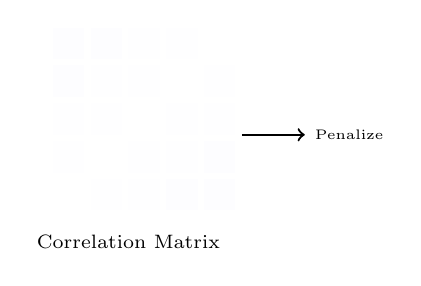
\begin{tikzpicture}[scale=0.8]
    % Correlation matrix visualization
    \foreach \i in {0,...,4} {
        \foreach \j in {0,...,4} {
            \pgfmathsetmacro{\corr}{abs(\i-\j)/5}
            \fill[blue!\corr!white] (\i*0.6,\j*0.6) rectangle ++(0.5,0.5);
        }
    }
    \node at (1.2,-0.5) {\scriptsize Correlation Matrix};
    \draw[->,thick] (3,1.2) -- (4,1.2) node[right] {\tiny Penalize};
\end{tikzpicture}
\end{center}
\end{columns}
\end{frame}

% Slide 8: QUBO Formulation
\begin{frame}{QUBO Formulation}
\textbf{Quadratic Unconstrained Binary Optimization:}

\begin{block}{Objective Function}
\begin{equation*}
\min_{x \in \{0,1\}^{520}} \quad Q(x) = \sum_{i} q_{ii}x_i + \sum_{i<j} q_{ij}x_ix_j + \text{offset}
\end{equation*}
\end{block}

\textbf{QUBO Matrix Components:}
\begin{enumerate}
    \item \textbf{Linear terms (diagonal):} Reward important APs
    \begin{equation*}
    q_{ii} = -\alpha \times \text{importance}_i^{\text{norm}}
    \end{equation*}

    \item \textbf{Quadratic terms (off-diagonal):} Penalize redundancy
    \begin{equation*}
    q_{ij} = (1-\alpha) \times \text{redundancy}_{ij}
    \end{equation*}

    \item \textbf{Constraint penalty:} Enforce exactly k APs selected
    \begin{equation*}
    \text{penalty} \times \left(\sum_{i} x_i - k\right)^2
    \end{equation*}
\end{enumerate}

\textbf{Parameters:} $k=20$, $\alpha=0.9$, penalty$=2.0$
\end{frame}

% Slide 9: Quantum-Inspired Solvers
\begin{frame}{Quantum-Inspired Solvers}
\begin{columns}
\column{0.5\textwidth}
\textbf{1. Simulated Quantum Annealing (SQA)}
\begin{itemize}
    \item Library: \texttt{OpenJij}
    \item Classical simulation of quantum effects
    \item Uses transverse field annealing
    \item Parameters:
    \begin{itemize}
        \scriptsize
        \item \texttt{num\_reads = 1000}
        \item \texttt{num\_sweeps = 1000}
    \end{itemize}
    \item Runtime: $\sim$52-57 seconds
\end{itemize}

\vspace{1em}
\textbf{2. Simulated Annealing (SA)}
\begin{itemize}
    \item Library: \texttt{D-Wave neal}
    \item Classical temperature-based search
    \item Parameters:
    \begin{itemize}
        \scriptsize
        \item \texttt{num\_reads = 1000}
        \item \texttt{beta\_range = (0.1, 5.0)}
    \end{itemize}
    \item Runtime: Comparable to SQA
\end{itemize}

\column{0.5\textwidth}
\textbf{Annealing Process:}
\begin{center}
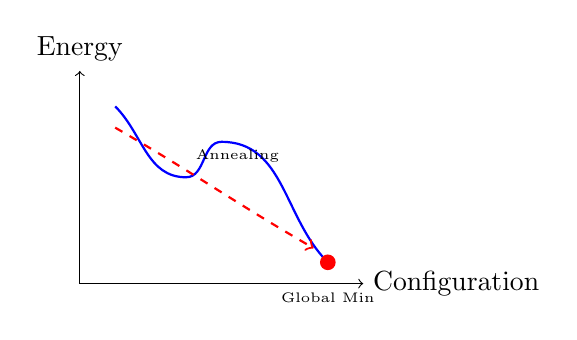
\begin{tikzpicture}[scale=0.9]
    % Energy landscape
    \draw[->] (0,0) -- (4,0) node[right] {Configuration};
    \draw[->] (0,0) -- (0,3) node[above] {Energy};

    % Landscape
    \draw[thick,blue] (0.5,2.5) to[out=-45,in=180] (1.5,1.5) to[out=0,in=180] (2,2) to[out=0,in=135] (3.5,0.3);

    % Global minimum
    \node[circle,fill=red,inner sep=2pt] at (3.5,0.3) {};
    \node[below] at (3.5,0) {\tiny Global Min};

    % Annealing path
    \draw[->,thick,red,dashed] (0.5,2.2) to[out=-30,in=150] (3.3,0.5);
    \node[right] at (1.5,1.8) {\tiny Annealing};
\end{tikzpicture}
\end{center}

\vspace{0.5em}
\textbf{Performance Metrics:}
\begin{itemize}
    \item Time-to-Solution (TTS)
    \item Success probability
    \item Solution diversity
    \item Energy convergence
\end{itemize}
\end{columns}
\end{frame}

% Slide 10: Machine Learning Post-Processing
\begin{frame}{Machine Learning: Random Forest}
\begin{columns}
\column{0.5\textwidth}
\textbf{Architecture:}
\begin{itemize}
    \item \textbf{Algorithm:} Random Forest Multi-Output Regressor
    \item \textbf{Trees:} 100 estimators
    \item \textbf{Max depth:} 12
    \item \textbf{Input:} RSSI from k=20 selected APs
    \item \textbf{Output:} 3D coordinates (LON, LAT, FLOOR)
\end{itemize}

\vspace{1em}
\textbf{Training:}
\begin{itemize}
    \item 19,937 training samples
    \item Out-of-Bag (OOB) validation
    \item OOB Score: \textbf{0.86 - 0.93}
\end{itemize}

\column{0.5\textwidth}
\begin{center}
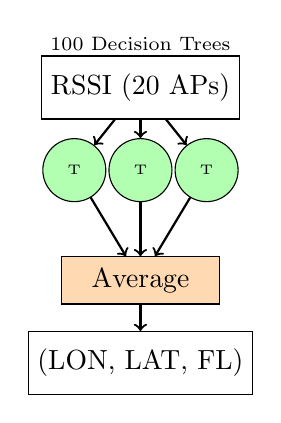
\begin{tikzpicture}[scale=0.7]
    % Input
    \node[draw,rectangle,minimum width=2cm,minimum height=0.8cm] (input) at (0,3) {RSSI (20 APs)};

    % Trees
    \foreach \x in {-1,0,1} {
        \node[draw,circle,fill=green!30,minimum size=0.8cm] (tree\x) at (\x*1.2,1.5) {\tiny T};
    }
    \node at (0,0.8) {$\vdots$};

    % Average
    \node[draw,rectangle,fill=orange!30,minimum width=2cm,minimum height=0.6cm] (avg) at (0,-0.5) {Average};

    % Output
    \node[draw,rectangle,minimum width=2cm,minimum height=0.8cm] (output) at (0,-2) {(LON, LAT, FL)};

    % Arrows
    \foreach \x in {-1,0,1} {
        \draw[->,thick] (input) -- (tree\x);
        \draw[->,thick] (tree\x) -- (avg);
    }
    \draw[->,thick] (avg) -- (output);

    \node[above] at (0,3.5) {\scriptsize 100 Decision Trees};
\end{tikzpicture}
\end{center}
\end{columns}

\vspace{0.5em}
\begin{block}{Advantages}
\begin{itemize}
    \item Handles non-linear relationships
    \item Robust to outliers
    \item Native multi-output support for 3D prediction
\end{itemize}
\end{block}
\end{frame}

% Slide 11: Results - Accuracy Comparison
\begin{frame}{Results: Accuracy by Importance Method}
\textbf{Performance with k=20 selected APs (Building 1):}

\begin{table}[h]
\centering
\small
\begin{tabular}{@{}lcccccc@{}}
\toprule
\textbf{Method} & \textbf{Mean Error} & \textbf{Median Error} & \textbf{Floor Acc.} & \textbf{OOB Score} & \textbf{QUBO Time} \\
& \textbf{(m)} & \textbf{(m)} & \textbf{(\%)} & & \textbf{(s)} \\
\midrule
\textcolor{blue}{\textbf{Average}} & \textcolor{blue}{\textbf{15.14}} & \textcolor{blue}{\textbf{11.38}} & 66.12 & 0.93 & 56.65 \\
Entropy & 15.99 & 11.76 & 58.96 & 0.91 & 54.20 \\
\textcolor{red}{\textbf{Max}} & 16.67 & 12.68 & \textcolor{red}{\textbf{69.06}} & 0.86 & 55.57 \\
Variance & 16.75 & 12.13 & 65.15 & 0.92 & 55.22 \\
Mutual Info & 19.65 & 13.63 & 62.87 & 0.89 & 51.97 \\
\bottomrule
\end{tabular}
\end{table}

\vspace{1em}
\textbf{Key Findings:}
\begin{itemize}
    \item \textcolor{blue}{\textbf{Average Importance}} achieves lowest mean/median error
    \item \textcolor{red}{\textbf{Max Importance}} achieves best floor accuracy (69.06\%)
    \item All methods significantly reduce dimensionality: 520 $\rightarrow$ 20 APs (\textbf{96\% reduction})
    \item Error range: 0.29m (best) to 83.5m (worst case)
    \item Consistent QUBO solution times ($\sim$52-57 seconds)
\end{itemize}
\end{frame}

% Slide 12: Results - Error Distribution
\begin{frame}{Results: Error Distribution Analysis}
\begin{columns}
\column{0.5\textwidth}
\textbf{3D Error Statistics (Average method):}
\begin{table}[h]
\centering
\scriptsize
\begin{tabular}{@{}lr@{}}
\toprule
\textbf{Metric} & \textbf{Value (m)} \\
\midrule
Mean Error & 15.14 \\
Median Error & 11.38 \\
Std Dev & 11.95 \\
Min Error & 0.29 \\
Max Error & 83.50 \\
90th Percentile & 29.72 \\
95th Percentile & 37.45 \\
\bottomrule
\end{tabular}
\end{table}

\vspace{0.5em}
\textbf{Floor Prediction:}
\begin{itemize}
    \item Correct floor: 66.12\%
    \item Off by 1 floor: $\sim$28\%
    \item Off by 2+ floors: $\sim$6\%
\end{itemize}

\column{0.5\textwidth}
\textbf{Error Breakdown:}
\begin{center}
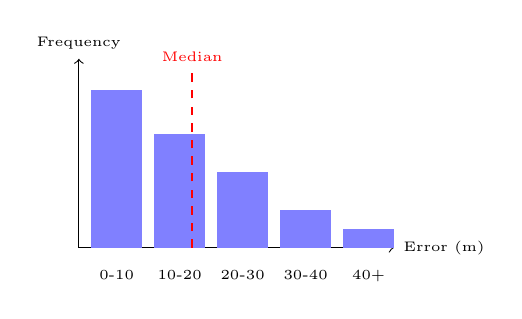
\begin{tikzpicture}[scale=0.8]
    % Histogram-like representation
    \draw[->] (0,0) -- (5,0) node[right] {\tiny Error (m)};
    \draw[->] (0,0) -- (0,3) node[above] {\tiny Frequency};

    \fill[blue!50] (0.2,0) rectangle (1,2.5);
    \fill[blue!50] (1.2,0) rectangle (2,1.8);
    \fill[blue!50] (2.2,0) rectangle (3,1.2);
    \fill[blue!50] (3.2,0) rectangle (4,0.6);
    \fill[blue!50] (4.2,0) rectangle (5,0.3);

    \node[below] at (0.6,-0.2) {\tiny 0-10};
    \node[below] at (1.6,-0.2) {\tiny 10-20};
    \node[below] at (2.6,-0.2) {\tiny 20-30};
    \node[below] at (3.6,-0.2) {\tiny 30-40};
    \node[below] at (4.6,-0.2) {\tiny 40+};

    \draw[red,thick,dashed] (1.8,0) -- (1.8,2.8) node[above] {\tiny Median};
\end{tikzpicture}
\end{center}

\vspace{0.5em}
\textbf{Observations:}
\begin{itemize}
    \item Right-skewed distribution
    \item 50\% of predictions $<$ 11.38m
    \item 90\% of predictions $<$ 29.72m
    \item Acceptable for indoor positioning
\end{itemize}
\end{columns}
\end{frame}

% Slide 13: Performance Analysis
\begin{frame}{Performance Analysis}
\begin{columns}
\column{0.5\textwidth}
\textbf{Computational Efficiency:}
\begin{itemize}
    \item \textbf{Dimensionality reduction:} 96.2\% (520 $\rightarrow$ 20 APs)
    \item \textbf{QUBO solving time:} $\sim$55 seconds
    \item \textbf{ML training:} $<$ 10 seconds
    \item \textbf{Prediction time:} Milliseconds per sample
\end{itemize}

\vspace{1em}
\textbf{Model Quality (Random Forest):}
\begin{itemize}
    \item OOB scores: 0.86 - 0.93
    \item Indicates excellent generalization
    \item Minimal overfitting
\end{itemize}

\vspace{1em}
\textbf{Solver Comparison:}
\begin{itemize}
    \item OpenJij SQA $\approx$ D-Wave SA
    \item Success probability: $>$ 80\%
    \item Stable convergence
\end{itemize}

\column{0.5\textwidth}
\textbf{Trade-offs Analysis:}

\begin{table}[h]
\centering
\scriptsize
\begin{tabular}{@{}lcc@{}}
\toprule
\textbf{Metric} & \textbf{520 APs} & \textbf{20 APs} \\
\midrule
Dimensionality & High & \textcolor{green}{Low} \\
Computation & Slow & \textcolor{green}{Fast} \\
Memory & High & \textcolor{green}{Low} \\
Mean Error & Lower & \textcolor{orange}{Higher} \\
Deployment & Complex & \textcolor{green}{Simple} \\
\bottomrule
\end{tabular}
\end{table}

\vspace{1em}
\begin{block}{Key Insight}
Acceptable accuracy trade-off for massive efficiency gain - ideal for resource-constrained IoT deployments
\end{block}
\end{columns}
\end{frame}

% Slide 14: Conclusions
\begin{frame}{Conclusions}
\textbf{Main Contributions:}
\begin{enumerate}
    \item \textbf{Novel QUBO formulation} for AP selection problem
    \begin{itemize}
        \item Balances importance and redundancy with parameter $\alpha$
        \item Adaptive penalty scaling for constraint enforcement
    \end{itemize}

    \item \textbf{Comprehensive method comparison}
    \begin{itemize}
        \item 6 importance metrics evaluated systematically
        \item Average and Max methods perform best
    \end{itemize}

    \item \textbf{Quantum-inspired optimization}
    \begin{itemize}
        \item Simulated Quantum Annealing achieves near-optimal solutions
        \item Comparable to classical approaches with potential quantum advantage
    \end{itemize}

    \item \textbf{Practical deployment solution}
    \begin{itemize}
        \item 96\% reduction in AP requirements
        \item Mean error 15.14m, Floor accuracy 69\%
        \item Suitable for real-world indoor positioning systems
    \end{itemize}
\end{enumerate}

\vspace{0.5em}
\begin{center}
\fbox{\parbox{0.9\textwidth}{\centering\textbf{Success:} Quantum-inspired optimization enables efficient, accurate indoor localization with minimal infrastructure}}
\end{center}
\end{frame}

% Slide 15: Future Work
\begin{frame}{Future Work \& Extensions}
\textbf{Short-term Enhancements:}
\begin{itemize}
    \item \textbf{Hyperparameter optimization:} Grid search for $\alpha$, penalty, $k$
    \item \textbf{Multi-building deployment:} Extend to all 3 buildings in dataset
    \item \textbf{Advanced ML models:} Deep learning, gradient boosting
    \item \textbf{Real-time updates:} Adaptive AP selection based on environment changes
\end{itemize}

\vspace{1em}
\textbf{Long-term Research:}
\begin{itemize}
    \item \textbf{True quantum hardware:} Deploy on D-Wave Advantage, IonQ
    \item \textbf{Hybrid quantum-classical algorithms:} QAOA, VQE
    \item \textbf{Dynamic optimization:} Time-varying QUBO for mobile scenarios
    \item \textbf{Multi-objective optimization:} Energy, cost, accuracy trade-offs
    \item \textbf{Transfer learning:} Generalize to new buildings without retraining
\end{itemize}

\vspace{1em}
\textbf{Practical Deployment:}
\begin{itemize}
    \item Field testing in real buildings
    \item Integration with commercial positioning systems
    \item Energy-efficient edge computing implementation
\end{itemize}
\end{frame}

% Thank you slide
\begin{frame}
\begin{center}
\Huge Thank You!

\vspace{2em}
\Large Questions?

\vspace{2em}
\normalsize
\textbf{Contact:} your.email@institution.edu

\vspace{0.5em}
\textbf{Code:} github.com/yourusername/Quantum-Optimization-In-AP-Selection
\end{center}
\end{frame}

\end{document}